\chapter{Maintenance}

This chapter explains how to maintain the {\em Catalog} and the {\em Janitor}
themselves.
It gives detailed instructions how to create new packages for the
Janitor.
To administrate the catalog, one can either use an ontology editor 
like Prot\`eg\`e, as explained in the next section, edit the documents
manually.
In the last section, a typical use case in maintaining the Janitor will
be presented.

% * Maintainance
% ** Protege and RDF files
% ** Creating own tar balls

\section{Catalog}\label{sec:catalog}

The Catalog describes runtime environments and is either served
through a web server or is distributed together with the Janitor as a
regular file.
It is specifed by a (Resource Description Framework) RDF file
assigned to the Janitor using the tag \texttt{catalog} within
the configuration file (see~\ref{sec:janitor_configuration}).
The format of the RDF file is defined by an RDF schema file
\texttt{knowarc.rdfs} which can be found along with an RDF
example file \texttt{knowarc.rdf} in the Janitor source directory
\href{http://svn.nordugrid.org/repos/nordugrid/arc1/trunk/src/services/janitor/resources/catalog/}
{http://svn.nordugrid.org/repos/nordugrid/arc1/trunk/src/services/janitor/resources/catalog/}.

To edit the catalog, the ontology editor Prot\`eg\`e may be
used. With some experience gained, one is likely to prefer a manual editing.
Figure~\ref{fig:protege_example} shows the editor while the
MetaPackage \texttt{APPS/BIO/JASPAR-CORE-1.0} of the example file has
been selected.

\begin{figure}
  \begin{center}
    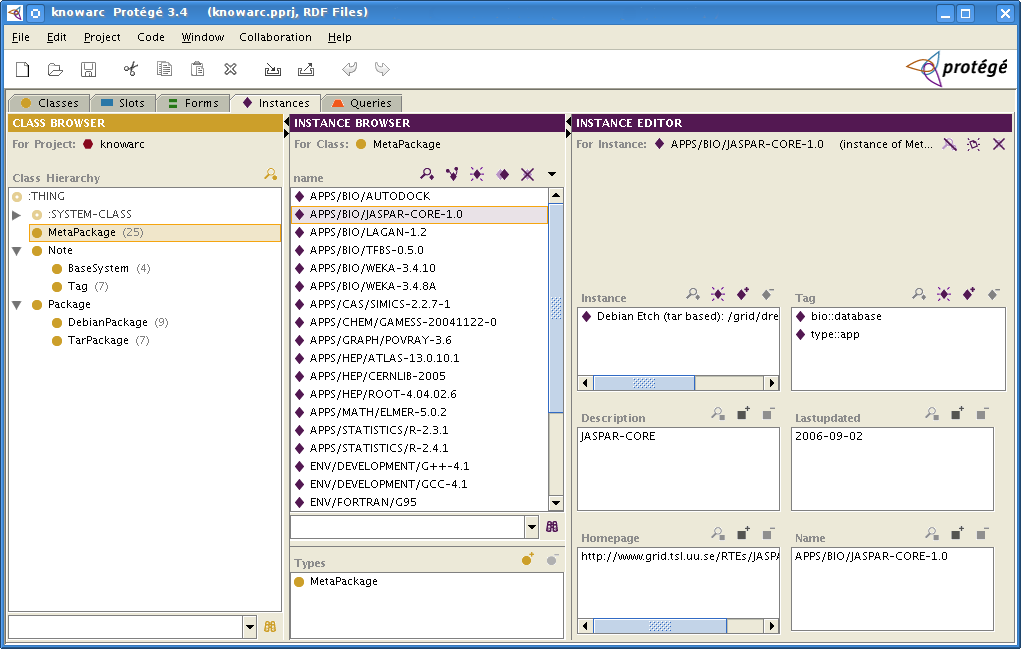
\includegraphics[width=\textwidth]{images/protege_JASPAR.png}
    \mycaption{Example of a RDF catalog file as displayed in the program Prot\`eg\`e.}{}
    \label{fig:protege_example}
  \end{center}
\end{figure}

On the left side of the editor the class browser is placed. Three
main classes are prepared: \texttt{MetaPackage}, \texttt{Note} and
\texttt{Package}. The RDF file is kept in the RDF:XML format, and
when inspecting the entry, one will fine a direct correspondence 
to the data stored in RDF:

\begin{verbatim}
<rdfs:Class rdf:about="&kb;MetaPackage"
         rdfs:label="MetaPackage">
  <rdfs:subClassOf rdf:resource="&rdfs;Resource"/>
  <rdfs:comment>
   Reference to a piece of software that shall be made available -
   somehow, and to the expectation to the grid user.  The traditional
   way to achieve the installation is via tarballs. Debian packages may
   be an alternative.
  </rdfs:comment>
</rdfs:Class>
<rdfs:Class rdf:about="&kb;Note"
   rdfs:label="Note">
   <rdfs:subClassOf rdf:resource="&rdfs;Resource"/>
</rdfs:Class>
<rdfs:Class rdf:about="&kb;Package"
   rdfs:label="Package">
  <rdfs:subClassOf rdf:resource="&rdfs;Resource"/>
  <rdfs:comment>
   Superclass of "TarPackage" and "DebianPackage".
  </rdfs:comment>
</rdfs:Class>
\end{verbatim}

The \texttt{Metapackage} is a general platform-independent description
of a \texttt{Package}. It can be understood as a reference to a functionality
that should be implemented at the remote site. But the exact instruction
on how to install it is not given.  The "instruction-level" comes with
instances of its subclass \texttt{Package}.

Links between resources are referred to as {\em Properties}. The following
specifies the dependencies that any package may have on other resources, i.e.
on other packages. The dependency on a base system is expressed by the
property {\em basesystem}, which not to be confused with the resource
{\em BaseSystem}.

\begin{verbatim}
<rdf:Property rdf:about="&kb;depends"
         rdfs:comment="lists dependencies of this package"
         rdfs:label="depends">
        <rdfs:domain rdf:resource="&kb;Package"/>
        <rdfs:range rdf:resource="&rdfs;Resource"/>
\end{verbatim}

MetaPackages contain one or more instances of the class
\texttt{Package}, which are then tangible software packages providing
the functionality that the MetaPackage references. The packages may
be aiming for different versions of the operating system or be different
in the way these are installed, but any package being assigned to the same
MetaPackage needs to perform the same functionality.
MetaPackages are described by the subclasses of \texttt{Note}, which
in turn has two subclasses: \texttt{BaseSystem} and
\texttt{Tag}.

The \texttt{MetaPackage} is described by the subclasses of \texttt{Note}.
The class \texttt{Note} has two subclasses: \texttt{BaseSystem} 
and \texttt{Tag} to describe the \texttt{MetaPackage}.

The \texttt{BaseSystem} describes the Debian release a \texttt{Package}
refers to (i.e. here etch or sid), i.e. the name of a common installation
or a virtual image.
The class \texttt{Tag} provides small keywords which can be assigned to
\texttt{MetaPackages} such that they can be found more easily.
\texttt{TarPackage} and \texttt{DebianPackage}
or currently the only subclasses of \texttt{Package}.

They are representing the necessary information (i.e. URL or Packagename)
for the installation.
To provide an overview on how the classes are
interacting with each other the Tables~\ref{tab:main_class_meta},
\ref{tab:main_class_base}, \ref{tab:main_class_tag},
\ref{tab:main_class_debian} and \ref{tab:main_class_tar} are pictured.

\begin{table}[!h]
   \begin{center}
        \mycaption{Specification of class \texttt{Metapackage}.}{}
         \label{tab:main_class_meta}
	\begin{tabular}{p{3cm}p{3cm}p{4cm}}
	\textbf{Name}  & \textbf{Cardinality}  & \textbf{Type}\\
	\hline
	description    & single                & String       \\
	homepage       & single                & String       \\
	instance       & multiple              & Instance of Package       \\
	lastupdated    & single                & String       \\
	name           & required single       & String       \\
	tag            & multiple              & Instance of Tag       \\
	\end{tabular} 
   \end{center}
\end{table}


\begin{table}[!h]
   \begin{center}
        \mycaption{Specification of class \texttt{BaseSystem}.}{}
         \label{tab:main_class_base}
	\begin{tabular}{p{3cm}p{3cm}p{4cm}}
	\textbf{Name}  & \textbf{Cardinality}  & \textbf{Type}\\
	\hline
	description    & single                & String       \\
	distribution   & required single       & String       \\
	name           & required single       & String       \\
	short\_description & required single   & String       \\
	url            & required single       & String       \\
	\end{tabular} 
   \end{center}
\end{table}


\begin{table}[!h]
   \begin{center}
        \mycaption{Specification of class \texttt{Tag}.}{}
         \label{tab:main_class_tag}
	\begin{tabular}{p{3cm}p{3cm}p{4cm}}
	\textbf{Name}  & \textbf{Cardinality}  & \textbf{Type}\\
	\hline
	description    & single                & String       \\
	name           & required single       & String       \\
	\end{tabular} 
   \end{center}
\end{table}

\begin{table}[!h]
   \begin{center}
        \mycaption{Specification of class \texttt{DebianPackage}.}{}
         \label{tab:main_class_debian}
	\begin{tabular}{p{3cm}p{3cm}p{6cm}}
	\textbf{Name}  & \textbf{Cardinality}  & \textbf{Type}\\
	\hline
	basesystem     & required single       & Instance of BaseSystem       \\
	debconf        & multiple              & String       \\
	depends        & multiple              & Instance of MetaPackage  or Package      \\
	package        & required multiple     & String      \\
	\end{tabular} 
   \end{center}
\end{table}

\begin{table}[!h]
   \begin{center}
        \mycaption{Specification of the class \texttt{TarPackage}.}{}
         \label{tab:main_class_tar}
	\begin{tabular}{p{3cm}p{3cm}p{6cm}}
	\textbf{Name}  & \textbf{Cardinality}  & \textbf{Type}\\
	\hline
	basesystem     & required single       & Instance of BaseSystem       \\
	depends        & multiple              & Instance of MetaPackage or Package      \\
	environ        & multiple              & String       \\
	url            & required multiple     & String      \\
	\end{tabular} 
   \end{center}
\end{table}

\subsection{Debian packages - dysfunctional in current implementation}

The problem with Debian packages is that these are available only for the
local machine and not immediately also for the whole network. This feature
was meant for setups that use virtual machines for the execution of jobs.

Those entries can also be used to help the specification of further
dependencies of runtime environments. It would then be left to the
responsibility of the system administrator to manually (or assisted with
scripts) distribute a series of extra Debian packages throughout the
compute nodes and use the catalog entry merely to indicate their presence.

One can as such interpret the catalog to represent an interface between
software distributed via Linux distributions and independently from these
via grid communities. It should be noted that the Linux distributions
have now all started to accept communities to maintain packages, which
may bringt many scientific packages away from being traditional ARC 
runtime environments towards becoming regular packages of some Linux
distribution. For Debian, the Debian-Science and
Debian-Med\footnote{\href{http://debian-med.alioth.debian.org}{http://debian-med.alioth.debian.org}}
communities are known to be very open to grid and cloud computing.

\section{HTML interface of the catalog}

The dynamic Runtime Environments stored in the
Catalog are presented on the aforementioned dedicated web
page\footnote{http://dre.knowarc.eu:8080/list.pl}. This site also
links to both the formal Catalog in RDF syntax and its automated
transformation to HTML. The latter mimics the traditional
site describing Runtime Environments in the Runtime Environment
Registry\footnote{http://gridrer.csc.fi/} in order to minimise issues
with an eventual transition to the new system.

That page, in a look resembling the classical description of RTE,
collects descriptions for Runtime Environments to encourage human site
administrators to install these.  This HTML page listing the manually or
automatically installable RTEs is prepared by the script web/list.pl.
This script is meant to be run by a mod-perl enabled Apache. The
script itself does not contribute to the core functionality of the
Janitor. It only performs the human-readable presentation of a catalog's
RDF file to users. In the first lines of the script some variables
specific to the site are set. To configure the script these have to be
changed~\cite[p. 9]{BAYER_2007}.

\section{Introducing new packages}\label{sec:introducing_new_packages}

This section describes how to add new packages to the Catalog. In
the current implementation, only tar based packages are processed by
the Janitor.  Within the here presented example they are assigned to
be used together with Debian Etch. This limitation is only literal.
There is no restriction for newer Debian distributions.

\subsection{Debian Etch (tar based)}

At the time of writing, only the tape archive (tar) file format is
accepted for dynamic Runtime Environment installation, a well accepted
file format throughout the UNIX community.
The concept reflects the
traditional manual approach towards RTE in ARC, for which one directory
is made available to all compute nodes.
This section explains the inner structure of the tar files for the
representation of dynamic runtime environments.  Subdirectories are
visualised in Figure~\ref{fig:tar_folder}.

\begin{figure}
  \begin{center}
    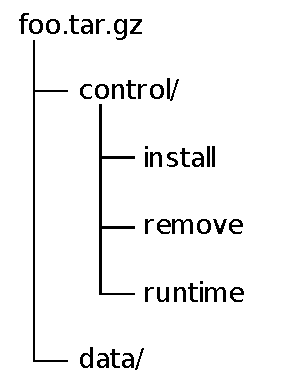
\includegraphics[width=4cm]{images/tar_folder.pdf}
    \mycaption{Directory structure in the tar files for automated installation.}{}
    \label{fig:tar_folder}
  \end{center}
\end{figure}

The tar file contains two directories, named {\tt control} and {\tt
data}:

\begin{description}
\item [data/] contains all software that the grid-job may need
\item [control/] contains files formally specifying how to deal
	with the information in the data/ directory.
\end{description}

Upon installation of such tar-based runtime environments,
the content of the data directory is extracted to some directory
\textdollar BAR.  After this unpacking of the tar file, the Janitor
executes the install script provided in the control directory.  It is
executed within the working directory \textdollar BAR. The job of
this skript is to perform any necessary post-processing.
The Janitor stores the file \texttt{control/remove}. It will be executed
in the same way as \texttt{control/install}, just before the tar-package
is removed. In most cases \texttt{control/remove} will be empty, implying
that the working directory \textdollar BAR shall be removed and no other
action is required.
Finally, the file \texttt{control/runtime} is sourced multiple times
by the Grid Manager's job-submit script. After installing the package,
the Janitor changes all occurences of \%BASEDIR\% in the runtime script
to \textdollar BAR.  Once the tar file was prepared, it must its entry
to a RTE Catalogue~\cite[p. 10]{BAYER_2007}.
But the working directory shall not be moved. All post-processing needs
to be performed \textit{in situ}.

From such Catalogs, the Janitor finds all information to install
packages that possibly have never been installed on the site before. The
offers of RTEs in a Catalog are cross-checked against the local
infrastructure and a subset of the available packages will be accepted as
"installable". This list of installable RTEs is forwarded to the grid
information system.

The remainder actions are regular actions performed upon execution of every grid-job. Upon submission,
the file \texttt{control/runtime} is sourced multiple times by the Grid Manager's job-submit script. Every
ARC runtime environment must specify such a runtime script, new is only its specific location as control/runtime.
Since the directory \textdollar BAR is not known for the individual preparing the runtime environment, that
file will instead use the placeholder \%BASEDIR\%.  After installing the package, the Janitor changes all
occurences of \%BASEDIR\% in the runtime script to \textdollar BAR.  To be offered to computing elements
for an installation, the such prepared runtime environment must be announced to a Catalog to which the
Janitor on the computing element subscribes~\cite[p. 10]{BAYER_2007}.

\subsection{Automated transformation of install directory to dRTE}

The script 'prepareDRE.pl' was created to help with the transformation
of a readily installed software into a dynamic runtime environment.
I also prepares a complete catalog file that can be offered
individually or next to other catalogs. See the associated man page
prepareDRE(8) for details.

\subsection{Protoypes}

In order to have an impression how the tar files are created, several
prototypes are provided at \url{http://dre.knowarc.eu}.

\subsubsection{Example: WEKA machine learning Java library}

The WEKA package for machine learning~\cite{FRANK_2004} and the Java
Runtime Environment are available as dynamic Runtime Environments. Further
packages for bioinformatics comprise dynamic variants of tools for
the analysis of transcription factor binding sites. These are already
offered for manual installation via the prior mentioned traditional page
representing Runtime Environments for ARC.
The \texttt{data} directory simply contains
a ZIP file which needs to be unzipped in the installation directory. For
that reason, the \texttt{control/install} script is written as follows:

% dollar signs made trouble in listings *hrmlgrmpf* ... Costs too much time to figure out why *ARC!*
\begin{verbatim} 
#!/bin/sh
set -e  # Makes the script to terminate at the first line it fails.

WEKA_ZIP="weka-3-4-8a.zip"
unzip $WEKA_ZIP
rm -f $WEKA_ZIP
\end{verbatim}
The runtime script sets the environment variable of the Java Classpath:
\begin{verbatim}
#!/bin/sh

WEKA_JAR="weka-3-4-8a/weka.jar"
case "\$1" in
	0)	# Just before job submission
		# none
	;;
	1)	# Just before job execution
		# Initialize the java environment
		CLASSPATH="%BASEDIR%/$WEKA_JAR:$CLASSPATH"
		export CLASSPATH
	;;
	2)	# After job termination
		# none
	;;
	*)
		return 1
	;;
esac	
\end{verbatim}

The remove script, which will be executed right before WEKA is
deinstalled, is empty. The Janitor will delete the whole directory,
so there remains nothing to be removed in addition.
The remove script may \eg be used to remove indices or other files
in /tmp.

%\subsection{Example: R packages in CRAN and BioConductor.org}
%\textbf{CRAN and BioConductor.org} To demonstrate the technical proximity to scientific communities that
%provide packages for the Debian Linux distribution, a tool was prepared to transform Debian packages to
%dynamic runtime environments\cite{MOELLER_2007}. This effort comprising more than 1700 packages and
%thus also helps to analyse the scalability of the RDF-based tool for the analysis of dependencies between
%projects.  \task{Why is CRAN and BioConductor.org mentioned here??}\\

\subsection{Example: ATLAS for High Energy Physics}

To address the concerns of the physicists using ARC, a dynamic runtime
environment for the ATLAS software suite was prepared. It extends prior
work on an automated installation that is available at
\href{http://guts.uio.no/atlas/12.0.6/}{http://guts.uio.no/atlas/12.0.6/}.

The preparation comprised the following steps:
\begin{itemize}
    \item The file system path specifications in the automated
       installation scripts were modified using the Janitor
       path variables.
    \item A tarball was prepared containing a directory structure as
       illustrated in Figure~\ref{fig:tar_folder}. The data directory
       was empty, since the automatic installation script downloads the
       software from a remote server.
    \item An entry was added to the Catalog file.
\end{itemize}

What sets High Energy Physics software apart is it's sheer size. The
package in question takes up more than 5 GB. This was a test illustrating
the feasibility of using dynamic RTEs in High Energy Physics. The
application of the dRTEs for ATLAS needs to wait for the planned web
service extension of the Catalog. With such a service, e.g. a software
manager of a big experiment will be able to deploy software packages
on production sites simply by creating a tarball and adding an entry to
the Catalog.

%\subsection{Debian Etch}
%
%These kind of packages are not yet supported.
%
%\subsection{Debian Sid}
%
%These kind of packages are not yet supported.
%
%\section{Adminstrating the Catalog}

%\section{Typical use cases}\label{sec:catalog}

% ** setstate REMOVAL_PENDING
% no warranty interferences in the file syste,

